\documentclass[11pt]{article}
\usepackage[latin1]{inputenc}
\usepackage{a4wide}
\usepackage{amsmath}
\usepackage{amsfonts}
\usepackage{amssymb}
\usepackage{graphicx}
\usepackage{enumerate}
\usepackage{epstopdf}
\usepackage{float}
\usepackage{multicol}
\usepackage{hyperref}
\epstopdfsetup{outdir=./images/}
\usepackage{subcaption}

\title{Natural Computing, Assignment 5}
\author{Dennis Verheijden - s4455770 \and Pauline Lauron - s1016609 \and Joost Besseling - s4796799}
\begin{document}
\maketitle

\section{}
\begin{enumerate}[(a)]
	\item A nash equilibrium occurs in the states $<S,S>$ and $<H,H>$. If we are in either of those states, no player can gain anything by changing their strategy, and in fact, they both lose 1.
	
	The candidate ESS's are the NE's, so both $<S,S>$ and $<H,H>$ are candidates. They both are ESS, since $P(S,S) = 1 > 0 = P(H,S)$ and $P(H,H) = 1 > 0 = P(S,H)$.
	
	\item Here, only the state $<S,S>$ is a strict Nash equilibrium. The state $<H,H>$ is a Nash equilibrium, since for both players, the best response to H has 0 payoff, although this payoff is gained by choosing either one of S or H. 
	
	The other states are not Nash equilibria, since the response to S should always be S (for both players, because of the symmetry of the game). $<S,S>$ is also an ESS because $P(S,S) = 1 > 0 = P(H,S)$.  
	
	\item In this game the only Nash equilibrium is $<S,S>$. The player changing to H will lose 1, so this is not the best response. And there is no ESS because $P(S,S) = 0 <  1 = P(H,S)$ and $P(H,H) = -20$ is the lowest value, so none of the condition is correct in order to be an ESS. 
	
	\item ESS are always Nash Equilibria, however this is not necessarily the case vice versa. % TODO : add more explanations with the relation between Nash equilibria and ESS.  
\end{enumerate}

\section{}
\begin{enumerate}[(a)]
	\item The ESSs of this game are $<A,A>$ and $<B,B>$ because $P(A,A) = 3 > 0 = P(B,A)$ and $P(B,B) = 1 > 0 = P(A,B)$.
	
	\item A two-player game with strategies A,B and payoffs :  $\pi(A,A) = 3 $, $\pi(A,B) = 0 $, $\pi(B, A) = 0 $, $\pi(B,B) = 1 $ and $x = $ proportion of individuals using A.
	\begin{enumerate}[i.]
		\item The expected payoff are the following : 
		\begin{itemize}
			\item $\pi(A,x) = 3x $
			\item $\pi(A,B) = 1-x$
		\end{itemize}
		
		\item
		\begin{align*}
		\dot{x} &= x(1-x)(\pi(A,x)-\pi(B,x)) \\
				&= x(1-x)(3x-(1-x)) \\
				&= x(1-x)(4x-1)
		\end{align*} 
		
		
		\item Fixed point $x* = 0$, $x* = 1$, $x* = 1/4$
		
		\item $x* = 1$, $x* = 0$ are the evolutionary end points because everyone uses strategy A or strategy B respectively. For  $x* = 1/4$, this is not stable. If there is more A, so the A replicate more fast than the B and in the other way, if there is more B, even if A has a bigger payoff, the B replicate faster than the A.
	\end{enumerate}
\end{enumerate}

\section{}
A two-player game with strategies H,D and payoffs :  $\pi(H,H) = 1/2(V-C) $, $\pi(H,D) = V $, $\pi(D,H) = 0 $, $\pi(D,D) = V/2 $
\begin{align*}
\dot{x} & = x(1-x)(1/2(V-C)x+V(1-x)-(V/2(1-x) \\
& = x(1-x)(V(1/2x+1-x-1/2+1/2x) + C(-1/2x)) \\
& = x(1-x)(1/2V - 1/2Cx)
\end{align*}
If we replace x with V/C, we obtain $\dot{x} = V/C*(1-V/C)(1/2*V-1/2*C*V/C) = 0$

\section{}
\begin{enumerate}[(a)]
	\item $v>2c$: Since the hawks will gain more than the doves, they will replicate faster than the doves. Since the doves gain nothing when they encounter a hawk, they will go extinct.
	
	$v \in [c,2c]$: Because the cost of fighting is relatively high, the hawks will gain too little when there are many other hawks. So the amount of hawks decreases until at some point they encounter more doves than hawks and the population stabilizes.
	
	$v<c$: The results is the same, but the ratio of hawks to doves changes.
	
	$v>2c$: After introduction of the retaliators, the retaliators replicate faster than the hawks, because they don't lose when they encounter one of their own. After a while the hawks go extinct (tried 10 times).
	
	$v=2c$: There is an unstable state, but after a while the hawk goes extinct. This is because the hawk cannot out compete the retaliator.
	
	\item We found the tool being fairly straightforward to use. Models can be easily loaded and you can graphically see what is going on. However, it can get chaotic very fast with many figures on the screen, such that it is easy to lose sight of what is going on.
\end{enumerate}

\newpage

\section{}
The two rules below. Since the black-white-black doesn't occur, both rules generate the same picture. 
\[ \LARGE
\substack{\blacksquare \blacksquare \blacksquare \\ \blacksquare} \enspace
\substack{\blacksquare \blacksquare \square \\ \square} \enspace
\substack{\blacksquare \square \blacksquare \\ \square } \enspace
\substack{\blacksquare \square \square \\ \square} \enspace
\substack{\square \blacksquare \blacksquare \\ \blacksquare} \enspace
\substack{\square \blacksquare \square \\ \square} \enspace
\substack{\square \square \blacksquare \\ \square} \enspace
\substack{\square \square \square \\ \square}
\]


\[ \LARGE
\substack{\blacksquare \blacksquare \blacksquare \\ \blacksquare} \enspace
\substack{\blacksquare \blacksquare \square \\ \square} \enspace
\substack{\blacksquare \square \blacksquare \\ \blacksquare } \enspace
\substack{\blacksquare \square \square \\ \square} \enspace
\substack{\square \blacksquare \blacksquare \\ \blacksquare} \enspace
\substack{\square \blacksquare \square \\ \square} \enspace
\substack{\square \square \blacksquare \\ \square} \enspace
\substack{\square \square \square \\ \square}
\]

\section{}
\begin{figure}[H]
	\centering
	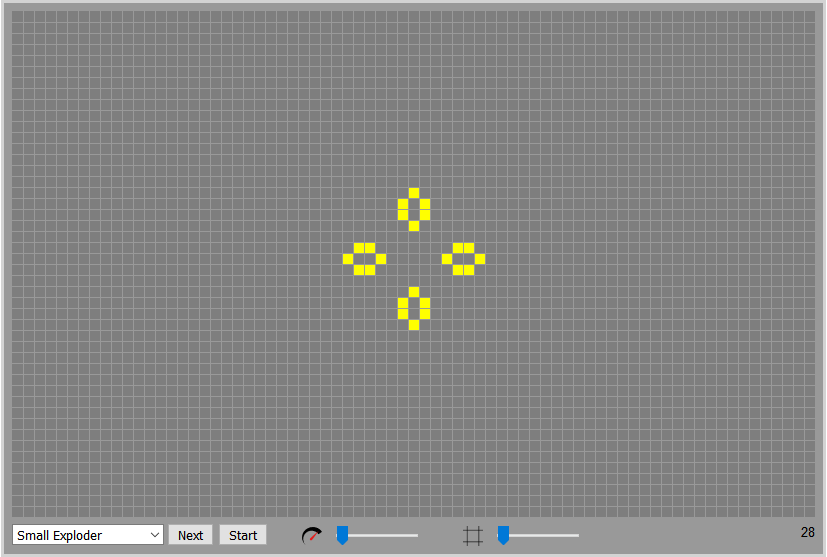
\includegraphics[width=0.7\textwidth]{images/q6.PNG}
	\caption{Small Exploder with a stable state.}
\end{figure}
This figure is static because for the space that is `populated', all of the cell have exactly 2 neighbors, so when we apply the rule ``Each cell with two or three neighbors survives", they survive with the same disposition.
Concerning the space that is `unpopulated', the maximum number of neighbords is less than 3, so by applying the rules, these cells stay empty. 
So when this configuration appears, it gets stuck because the ``old" cells survive and none of the other cells become populated. 

\end{document}